% SVN info for this file
\svnidlong
{$HeadURL$}
{$LastChangedDate$}
{$LastChangedRevision$}
{$LastChangedBy$}

\chapter{Il gruppo fondamentale}
\labelChapter{gruppofonduta}

\begin{introduction}
	‘‘BEEP BOOP INSERIRE CITAZIONE QUA BEEP BOOP.''
	\begin{flushright}
		\textsc{NON UN ROBOT,} UN UMANO IN CARNE ED OSSA BEEP BOOP.
	\end{flushright}
\end{introduction}

\section{Omotopie fra cammini}
Ove non specificato differentemente, useremo $I$ per indicare l'intervallo $\intv$.
\begin{define}
	Siano $\funz{\alpha,\ \beta}{I}{X}$ due cammini da $a$ a $b$, cioè con \textit{stessi estremi}. Allora $\alpha\,\beta$ sono \textbf{cammini omotopi}\index{cammino!omotopo} se $\exists \funz{F}{I \times I}{X}$ tale che:
	\begin{equation}
		\begin{array}{ll}
			\begin{cases}
							\mvf{F}{t}{0}=\alpha\left(t\right)\\
				\mvf{F}{t}{1}=\beta\left(t\right)
			\end{cases}&
		\forall t\in I\ \text{ è omotopia tra } \alpha \text{ e }\beta\\
			\begin{cases}
			\mvf{F}{0}{s}=a\\
			\mvf{F}{1}{s}=b
		\end{cases}&
		\forall s\in I\ \mvf{F}{\bullet}{s} \text{ è sempre un cammino tra } a \text{ e }b
		\end{array}
	\end{equation}
$F$ è detta \textbf{omotopia di cammini}\index{omotopia!di cammini} o \textbf{omotopia a estremi fissi} \seeonlyindex{omotopia!a estremi fissi}{omotopia!di cammini}.
\end{define}
\begin{define}
	Indichiamo con $\inscam{X}{a}{b}$ l'insieme dei cammini in $X$ da $a$ a $b$.
\end{define}
\begin{observe}
	L'omotopia di cammini è una relazione di equivalenza su $\inscam{X}{a}{b}$.
\end{observe}
\begin{demonstration}~{}
		\begin{itemize}
		\item \textsc{Riflessiva}: $\alpha\sim \alpha ?$. Presa $\mvf{F}{t}{s}=\alpha\left(t\right)$, essa è ben definita, continua e:
		\begin{equation*}
			\mvf{F}{t}{0}=\alpha\left(t\right),\ \mvf{F}{t}{1}=\alpha\left(t\right),\ \mvf{F}{0}{s}=\alpha\left(0\right)=a,\ \mvf{F}{1}{s}=\alpha\left(1\right)=b
		\end{equation*}
	Cioè è omotopia di cammini tra $\alpha$ e se stessa.
		\item \textsc{Simmetrica}: Da $\alpha\sim \beta$ sappiamo che esiste $F$ omotopia di cammini per cui:
		\begin{equation*}
			\mvf{F}{t}{0}=\alpha\left(t\right),\ \mvf{F}{t}{1}=\beta\left(t\right),\ \mvf{F}{0}{s}=a,\ \mvf{F}{1}{s}=b
		\end{equation*}
		Per avere $\beta\sim \alpha$, basta prendere $\mvf{\tilde{F}}{t}{s}=\mvf{F}{t}{1-s}$: essa è ben definita, continua e:
		\begin{gather*}
			\mvf{\tilde{F}}{t}{0}=\mvf{F}{t}{1}=\beta\left(t\right),\ \mvf{\tilde{F}}{t}{1}=\mvf{F}{t}{0}=\alpha\left(t\right)\\ \mvf{\tilde{F}}{0}{s}=\mvf{F}{0}{s}=a,\ \mvf{\tilde{F}}{1}{s}=\mvf{F}{1}{s}=b
		\end{gather*}
		Cioè è omotopia di cammini tra $\beta$ e $\alpha$.
		\item \textsc{Transitiva}: Da $\alpha\sim \beta$ abbiamo:
	\begin{equation*}
			\begin{array}{ll}
			\begin{cases}
				\mvf{F}{t}{0}=\alpha\left(t\right)\\
				\mvf{F}{t}{1}=\beta\left(t\right)
			\end{cases}&
		\begin{cases}
				\mvf{F}{0}{s}=a\\
				\mvf{F}{1}{s}=b
		\end{cases}
			\end{array}
	\end{equation*}
Mentre da $\beta\sim \gamma$:
	\begin{equation*}
	\begin{array}{ll}
		\begin{cases}
			\mvf{G}{t}{0}=\beta\left(t\right)\\
			\mvf{G}{t}{1}=\gamma\left(t\right)
		\end{cases}&
	\begin{cases}
			\mvf{G}{0}{s}=a\\
			\mvf{G}{1}{s}=b
	\end{cases}
	\end{array}
\end{equation*}
Definita allora la seguente funzione:
\begin{equation*}
	\mvf{H}{t}{s}=\begin{cases}
		\begin{array}{ll}
			\mvf{F}{t}{2s}&\text{se }s\in\left[0,\ \frac{1}{2}\right]\\
			\mvf{G}{t}{2s-1}&\text{se }s\in\left[\frac{1}{2},\ 1\right]
		\end{array}
	\end{cases}
\end{equation*}
Essa è ben definita, continua per il lemma di incollamento e tale per cui:
\begin{gather*}
	\mvf{H}{t}{0}=\mvf{F}{t}{0}=\alpha\left(t\right),\ \mvf{H}{t}{1}=\mvf{G}{t}{1}=\gamma\left(t\right)\\
	\mvf{H}{0}{s}=a,\ \mvf{H}{1}{s}=b
\end{gather*}
		Cioè è omotopia di cammini tra $\alpha$ e $\gamma$.
	\end{itemize}
\end{demonstration}
\begin{remember}
Abbiamo già definito due ‘‘operazioni'' fra insiemi di cammini, senza averle necessariamente formalizzate:
\begin{itemize}
\item \textsc{Prodotto di cammini}: $\funztot{\ }{\inscam{X}{a}{b}\times\inscam{X}{b}{c}}{\inscam{X}{a}{c}}{\left(\alpha,\ \beta\right)}{\alpha\ast\beta}$
\item \textbf{Inversione di cammini}: $\funztot{\ }{\inscam{X}{a}{b}}{\times\inscam{X}{b}{a}}{\alpha}{\overline{\alpha}}$
\end{itemize}
\end{remember}
\begin{observe}
Si ha $\overline{\overline{\alpha}}=\alpha$. Infatti:
\begin{equation*}
	\overline{\alpha}\left(t\right)=\alpha\left(1-t\right)\implies\overline{\overline{\alpha}}\left(t\right)=\overline{\alpha}\left(1-t\right)=\alpha\left(t\right)
\end{equation*}
\vspace{-6mm}
\end{observe}
\begin{lemming}\textsc{Composizioni di omotopie di cammini (Kosniowski, 14.2)\label{compoomotopecammini}}\\
	Dati $\alpha,\ \alpha'\in\inscam{X}{a}{b}$ e $b,\ b'\in\inscam{X}{b}{c}$, parlando in termini di omotopie di cammini:
	\begin{equation}
		\alpha\sim \alpha'\text{ e }\beta\sim \beta'\implies \alpha\ast\beta\sim\alpha'\ast\beta'
	\end{equation}
\vspace{-6mm}
\end{lemming}
\begin{demonstration}
	Esistono $\funz{F,\ G}{I\times I}{X}$ tali che:
	\begin{gather*}
		\begin{array}{ll}
			\mvf{F}{t}{0}=\alpha\left(t\right)&\mvf{F}{0}{s}=a\\
			\mvf{F}{t}{1}=\alpha'\left(t\right)&\mvf{F}{1}{s}=b
		\end{array}
	\forall t,\ s\in I\\
		\begin{array}{ll}
	\mvf{G}{t}{0}=\beta\left(t\right)&\mvf{G}{0}{s}=b\\
	\mvf{G}{t}{1}=\beta'\left(t\right)&\mvf{G}{1}{s}=c
\end{array}	
	\forall t,\ s\in I
	\end{gather*}
Consideriamo $\funz{H}{I\times I}{X}$ data da:
\begin{equation*}
	\mvf{H}{t}{s})\begin{cases}
				\begin{array}{lc}
			\mvf{F}{2t}{s} & \text{se }0\leq t\leq \frac{1}{2}\\
			\mvf{F}{2t-1}{s} & \text{se }\frac{1}{2}\leq t\leq 1	
		\end{array}
	\end{cases}
\end{equation*}
\begin{itemize}
	\item $H$ è ben definita per $t=\frac{1}{2}$
	\item $H$ è continua per il lemma di incollamento, essendo definito sui chiusi $\left[0,\ \frac{1}{2}\right]\times I$ e $\left[\frac{1}{2},\ 1\right]\times I$ è continua su di essi.
\item \parbox[t]{0.25\textwidth}{$\mvf{H}{t}{0}=\left(\alpha\ast\beta\right)\left(t\right)$}\tikzmark{a}
\item \parbox[t]{0.25\textwidth}{$\mvf{H}{t}{1}=\left(\alpha'\ast\beta'\right)\left(t\right)\ $}\tikzmark{b}
\item \parbox[t]{0.25\textwidth}{$\mvf{H}{0}{s}=\mvf{F}{0}{0}=a$}\tikzmark{c}
\item \parbox[t]{0.25\textwidth}{$\mvf{H}{1}{s}=\mvf{G}{1}{0}=c$}\tikzmark{d}
\end{itemize}
\brackitem{a}{b}[$\forall t\in I$ è omotopia]
\brackitem{c}{d}[$\forall s\in I$ ha estremi fissi]
$H$ è l'omotopia a estremi fissi cercata.
\end{demonstration}
\begin{lemming}\textsc{Cambiamento di parametri (Manetti, 11.3)}\\
	Sia $\funz{\alpha}{I}{X}$ un cammino e $\funz{\varphi}{I}{I}$ una funzione continua tale che $\varphi\left(0\right)=0$ e $\varphi\left(1\right)=1$. Allora $\alpha\circ \varphi\sim\alpha$.
\end{lemming}
\begin{demonstration}
	Sia $\funz{F}{I\times I}{X}$ data da $\mvf{F}{t}{s}=\alpha\left(s\varphi\left(t\right)+\left(1-s\right)t\right)$.
	\begin{itemize}
		\item $s\varphi\left(t\right)+\left(1-s\right)t$ è una combinazione lineare che è contenuta in $I\subseteq \realset\ \forall t,\ s\in I$ per convessità dell'intervallo $I$, da cui segue che $F$ è ben definita.
		\item $F$ continua perché composizione di funzioni continue.
		\item \parbox[t]{0.38\textwidth}{$\mvf{F}{t}{0}=\alpha\left(t\right)$}%\tikzmark{a}
		\item \parbox[t]{0.38\textwidth}{$\mvf{F}{t}{1}=\alpha\left(\varphi\left(t\right)\right)$}%\tikzmark{b}
		\item \parbox[t]{0.38\textwidth}{$\mvf{F}{0}{s}=\alpha\left(0\right)$}%\tikzmark{c}
		\item \parbox[t]{0.38\textwidth}{$\mvf{F}{1}{s}=\alpha\left(s+1-s\right)=\alpha\left(1\right)$}%\tikzmark{d}
	\end{itemize}
%\brackitem{a}{b}[$\forall t\in I$ è omotopia]
%\brackitem{c}{d}[$\forall s\in I$ ha estremi fissi]
$H$ è l'omotopia a estremi fissi cercata tra $\alpha$ e $\alpha\circ\varphi$.
\end{demonstration}
\begin{define}
	Il \textbf{cammino costante} $C_a$\index{cammino!costante} nel punto $a$ è un cammino che non si sposta mai da esso, cioè è descritto da una funzione costante nel punto:
	\begin{equation}
		\funztot{C_a}{I}{X}{t}{a}
	\end{equation}
\vspace{-6mm}
\end{define}
\begin{proposition}\textsc{(Manetti, 11.4 e 11.6)\label{propcammini}}\\
	Sia $X$ spazio topologico e si considerino i cammini:
	\begin{equation*}
	\alpha\in\inscam{X}{a}{b}\quad\beta\in\inscam{X}{b}{c}\quad\gamma\in\inscam{X}{c}{d}
	\end{equation*}
Valgono le seguenti proprietà:
\begin{enumerate}
	\item \textsc{Associatività}: $\left(\alpha\ast\beta\right)\ast \gamma \sim \alpha\ast\left(\beta\ast\gamma\right)$.
	\item \textsc{Rapporto coi cammini costanti}: $C_a\ast \alpha \sim \alpha \sim \alpha \ast C_b$. 
	\item \textsc{Inverso}: $\alpha\ast\overline{\alpha}\sim C_a$ e $\overline{\alpha}\ast\alpha\sim C_a$.
\end{enumerate}
\end{proposition}
\begin{demonstration}~{}
\begin{enumerate}[label=\Roman*]
	\item Scriviamo i due cammini:
	\begin{gather*}
\left(\left(\alpha\ast\beta\right)\ast\gamma\right)\left(t\right)=\begin{cases}
	\begin{array}{ll}
		\alpha\left(4t\right)&t\in\left[0,\ \frac{1}{4}\right]\\
		\beta\left(4t-1\right)&t\in\left[\frac{1}{4},\ \frac{1}{2}\right]\\
		\gamma\left(2t-1\right)&t\in\left[\frac{1}{2},\ 1\right]
	\end{array}
\end{cases}\\
\left(\left(\alpha\ast\left(\beta\gamma\right)\right)\right)\left(t\right)=\begin{cases}
\begin{array}{ll}
	\alpha\left(2t\right)&t\in\left[0,\ \frac{1}{2}\right]\\
	\beta\left(4t-2\right)&t\in\left[\frac{1}{2},\ \frac{3}{4}\right]\\
	\gamma\left(2t-3\right)&t\in\left[\frac{3}{4},\ 1\right]
\end{array}
\end{cases}
	\end{gather*}
I due cammini differiscono per una \textit{riparametrizzazione} $\funz{\oldphi}{I}{I}$ di $\alpha\ast\left(\beta\ast\gamma\right)$ definita in questo modo:
\begin{gather*}
	\begin{cases}
		\begin{array}{l}
			2s=4t\\
			4s-2=4t-2\\
			4s-3=4t-1
		\end{array}
\implies
\begin{cases}
\begin{array}{ll}
	s=2t&t\in\left[0,\ \frac{1}{2}\right]\\
	s=t+\frac{1}{4}&t\in\left[\frac{1}{4},\ \frac{1}{2}\right]\\
	s=\frac{t}{2}+\frac{1}{2}&t\in\left[\frac{1}{2},\ 1\right]
\end{array}
		\end{cases}
	\end{cases}\\
\oldphi\left(t\right)=	\begin{cases}
\begin{array}{ll}
	2t&t\in\left[0,\ \frac{1}{2}\right]\\
	t+\frac{1}{4}&t\in\left[\frac{1}{4},\ \frac{1}{2}\right]\\
	\frac{t}{2}+\frac{1}{2}&t\in\left[\frac{1}{2},\ 1\right]
\end{array}
		\end{cases}
\end{gather*}
\begin{itemize}
	\item $\oldphi$ è ben definita e continua per lemma di incollamento.
	\item $\oldphi\left(0\right)=0$ e $\oldphi\left(1\right)=1$.
	\item $\left(\left(\alpha\ast\left(\beta\ast\gamma\right)\right)\right)\left(\oldphi\left(t\right)\right)=\left(\left(\alpha\ast\beta\right)\ast\gamma\right)\left(t\right)$.
\end{itemize}
Per il lemma del cambiamento di variabile i due cammini sono omotopi.
\item Scriviamo i due cammini:
\begin{gather*}
	\left(C_a\ast \alpha\right)\left(t\right)=\begin{cases}
		\begin{array}{ll}
			a&t\in\left[0,\ \frac{1}{2}\right]\\
			\alpha\left(2t-1\right)&t\in\left[\frac{1}{2},\ 1\right]
		\end{array}
	\end{cases}\\
	\left(\alpha\ast C_b\right)\left(t\right)=\begin{cases}
		\begin{array}{ll}
			\alpha\left(2t\right)&t\in\left[0,\ \frac{1}{2}\right]\\
			b&t\in\left[\frac{1}{2},\ 1\right]
		\end{array}
	\end{cases}
\end{gather*}
I due cammini differiscono per delle \textit{riparametrizzazioni} di $\alpha$ $\funz{\oldphi}{I}{I}$ e $\funz{\psi}{I}{I}$ definite così:
\begin{equation*}
	\oldphi\left(t\right)=
	\begin{cases}
		\begin{array}{ll}
			0&t\in\left[0,\ \frac{1}{2}\right]\\
			2t-1&t\in\left[\frac{1}{2},\ 1\right]
		\end{array}
	\end{cases}
\qquad	\psi\left(t\right)=
\begin{cases}
	\begin{array}{ll}
		2t&t\in\left[0,\ \frac{1}{2}\right]\\
		1&t\in\left[\frac{1}{2},\ 1\right]
	\end{array}
\end{cases}
\end{equation*}
\begin{itemize}
	\item $\oldphi$ e $\psi$ son ben definite e continue per lemma di incollamento.
	\item $\oldphi\left(0\right)=0,\ \psi\left(0\right)=0$ e $\oldphi\left(1\right)=1,\psi\left(1\right)=1 $.
	\item $\left(C_a\ast \alpha\right)\left(t\right)=\alpha\left(\oldphi\left(t\right)\right)$ e $\left(\alpha\ast C_b\right)\left(t\right)=\alpha\left(\psi\left(t\right)\right)$.
\end{itemize}
Per il lemma del cambiamento di variabile i due cammini sono entrambi omotopi a $\alpha$, si hanno quindi le equivalenze omotopiche cercate.
\item È sufficiente dimostrare che $\alpha\ast\overline{\alpha}\sim C_a$. Possiamo immaginare di rappresentare tutte le parametrizzazioni di cammini definiti da un omotopia sul piano $I\times I$, con $t$ sulle ascisse e $s$ sulle ordinate.\\
In questo modo i punti $a$ di inizio e $b$ di fine sono rappresentati dai segmenti verticali in $t=0$ e in $t=1$, mentre i cammini $\alpha$ di inizio e $\beta$ fine sono segmenti orizzontali in $s=0$ e $s=1$. Dunque, all'interno di $I\times I$ possiamo  trovare (fissato $s$) tutti i cammini $\mvf{F}{\bullet}{s}$ di estremi $a$ e $b$ compresi tra i cammini $\alpha$ e $\beta$: essi sono rappresentati da segmenti orizzontali.\\
\begin{minipage}{.62\linewidth}
Nel nostro caso, possiamo considerare il punto $a$ di inizio e il punto $b$ di fine del cammino $\alpha$. Nei due cammini ‘‘esterni'' o il cammino non si sposta mai da $a$ ($C_a$), oppure percorre tutto il cammino $\alpha$ fino a $b$ (che è raggiunto per $t=\frac{1}{2}$) e torna poi indietro per lo \textit{stesso cammino} ($\alpha\ast\overline{\alpha}$). Tuttavia, dobbiamo considerare anche cammini che percorrono $\alpha$ fino ad un punto $c$ \textit{intermedio} fra $a$ e $b$, stanno fermi in $c$ per poi tornare indietro. Definiamo la seguente omotopia:
\end{minipage}
\begin{minipage}{.37\linewidth}
	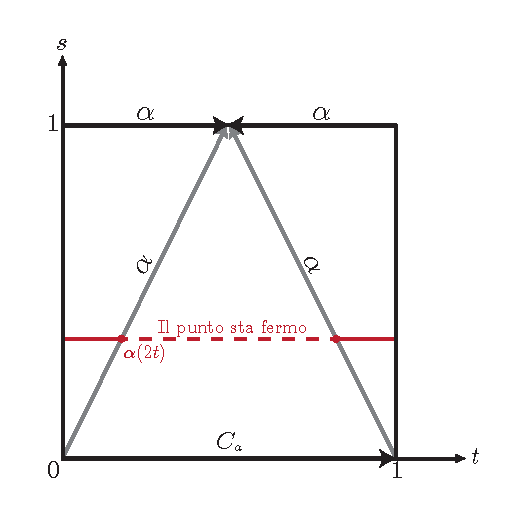
\includegraphics[trim=0cm 0cm 0cm 0cm,clip,scale=0.6]{images/camminoinverso.pdf}
\end{minipage}
\begin{equation}
	\mvf{F}{t}{s}=\begin{cases}
		\begin{array}{ll}
			\alpha\left(2t\right)&\text{se }0\leq t\leq \frac{s}{2}\\
			\alpha\left(s\right)&\text{se }\frac{s}{2}\leq t\leq 1-\frac{s}{2}\\
			\alpha\left(2-2t\right)&\text{se }1-\frac{s}{2}\leq t\leq 1
		\end{array}
	\end{cases}
\end{equation}
Verifichiamo che lo sia:
\begin{itemize}
\item $F$ è ben definita grazie alla ben definizione di $\alpha$: tutti i valori di $F$ risultano interni ad $X$.
\item $F$ è continua per il lemma di incollamento.
\item $\mvf{F}{t}{0}=\alpha\left(0\right)=C_a\left(t\right),\ \mvf{F}{t}{1}=\alpha\ast\overline{\alpha}\left(t\right)$ e $\mvf{F}{0}{s}=a=\mvf{F}{1}{s}$.
\end{itemize}
In questo modo teniamo conto della possibilità del cammino di ‘‘fermarsi'' per un certo tempo in un particolare punto $\alpha\left(s\right)$. 
\end{enumerate}
\end{demonstration}
\section{Gruppo fondamentale}
\begin{define}
	Sia $X$ uno spazio topologico e fissiamo un punto $x_0\in X$. I \textbf{lacci}\index{laccio} o \textbf{cappi}\seeonlyindex{cappio}{laccio} sono i cammini chiusi in $X$, cioè tutti i cammini il cui punto iniziale e finale coincidono. Il loro insieme si denota dunque come $\inscam{X}{x_0}{x_0}$.
\end{define}
\begin{observe}
	Possiamo notare come $\forall\alpha,\ \beta\in\inscam{X}{x_0}{x_0}$ si ha:
	\begin{equation*}
		\alpha\ast\beta\in\inscam{X}{x_0}{x_0}\qquad \overline{\alpha}\in\inscam{X}{x_0}{x_0}
	\end{equation*}
Allora, se quozientiamo l'insieme dei lacci rispetto alla relazione di equivalenza data dall'omotopia di cammini, esso possiede una struttura di \textit{gruppo}:
\begin{equation}
	\begin{array}{cc}
	\gruf{X}{x_0}=&\frac{\inscam{X}{x_0}{x_0}}{\sim}
	\end{array}	
\end{equation}
Preso un laccio $\alpha$, indichiamo la sua classe di equivalenza in $\gruf{X}{x_0}$ con $\left[\alpha\right]$. Allora:
\begin{itemize}
	\item Il prodotto di cammini dà un operazione ben definita su $\gruf{X}{x_0}$ grazie al lemma \ref{compoomotopecammini} (Kosniowski, 14.2):
	\begin{equation}
		\left[\alpha\right]\cdot\left[\beta\right]=\left[\alpha\ast\beta\right]
	\end{equation}
\item L'operazione appena definita è associativa per il primo punto della proposizione \ref{propcammini} (Manetti, 11.4 e 11.6).
\item $\left[C_{x_0}\right]$ è l'elemento neutro, sempre per la proposizione \ref{propcammini} (Manetti, 11.4 e 11.6):
\begin{equation}
	\left[C_{x_0}\right]\cdot\left[\alpha\right]=\left[\alpha\right]=\left[\alpha\right]\cdot\left[C_{x_0}\right]
\end{equation} 
\item $\left[\overline{\alpha}\right]$ è l'inverso di $\left[\alpha\right]$, cioè $\left[\alpha\right]^{-1}\coloneqq\left[\overline{\alpha}\right]$, per la proposizione \ref{propcammini} (Manetti, 11.4 e 11.6):
\begin{equation}
\left[\overline{\alpha}\right]\cdot\left[\alpha\right]=\left[C_{x_0}\right]=\left[\alpha\right]\cdot\left[\overline{\alpha}\right]
\end{equation}
\end{itemize}
\vspace{-6mm}
\end{observe}
\begin{attention}
	La proposizione \ref{propcammini} (Manetti, 11.4 e 11.6) ci garantisce che la composizione di cammini omotopi è omotopa ($\left(\alpha\ast\beta\right)\ast \gamma \sim \alpha\ast\left(\beta\ast\gamma\right)$), dunque possiamo parlare della \textit{classe} $\left[\alpha\ast\beta\ast\gamma\right]$. Tuttavia, al di fuori del quoziente non ha senso $\alpha\ast\beta\ast\gamma$!\\
	L'ordine con cui congiungiamo i cammini dà luogo a due cammini certamente omotopi, \textit{ma non uguali}, dato che la parametrizzazione varia\footnote{Questo si vede chiaramente nella dimostrazione della proposizione.}.
\end{attention}
\begin{define}
	Dato uno spazio topologico $X$ e fissato un punto (detto \textbf{punto base}\index{punto!base}) $x_0$, il \textbf{gruppo fondamentale}\index{gruppo!fondamentale} con punto base $x_0$ è il gruppo $\gruf{X}{x_0}$ definito nell'osservazione precedente.\\
	Si chiama anche \textbf{primo gruppo fondamentale}\index{gruppo!fondamentale!primo} o \textbf{gruppo di Poincaré}\seeonlyindex{gruppo!di Poicaré}{gruppo!fondamentale}.
\end{define}
\subsection{Dipendenza dal punto base}
\begin{theorema}\label{dipendenzaptobasegruf}
	Il gruppo fondamentale dipende \textit{solo} dalla componente \textit{c.p.a.} contente il punto base $x$.\\
	In altre parole, se $x,\ y\in X$ appartengono alla stessa componente \textbf{c.p.a.}, preso un arco $\gamma$ da $x$ a $y$ e costruito:
	\begin{equation}
		\funztot{\gamma_{\#}}{\gruf{X}{x}}{\gruf{X}{y}}{\left[\alpha\right]}{\left[\overline{\gamma}\ast\alpha\ast\gamma\right]}
	\end{equation}
	È ben definito ed è un \textit{isomorfismo} di gruppi, cioè:
	\begin{equation}
		\gruf{X}{x}\cong\gruf{X}{y}
	\end{equation}
\vspace{-6mm}
\end{theorema}
\begin{remember}
	Una funzione fra due gruppi $\funz{f}{\left(G,\ \cdot_G\right)}{\left(H,\ \cdot_H\right)}$ è un \textbf{omomorfismo di gruppi}\index{omomorfismo di gruppi} se:
	\begin{gather*}
		f\left(a\cdot_G b\right)=f\left(a\right)\cdot_H f\left(b\right)\quad \forall a,\ b\in G
	\end{gather*}
	Se $f$ è \textit{biettiva}, allora parliamo di \textbf{isomorfismo di gruppi}\index{isomorfismo di gruppi}.
\end{remember}
\begin{demonstration}~{}
	\begin{itemize}
		\item $\gamma_{\#}$ è ben definito in quanto la classe $\left[\overline{\gamma}\ast\alpha\ast\gamma\right]$ è ben definita per la composizione dei cammini ed è la classe di equivalenza di un cappio di $y$ ($\overline{\gamma}$ parte da $y$ e raggiunge $x$, con $\alpha$ compie un cammino chiuso in $x$ per tornare al punto di partenza $y$).
		\item $\gamma_{\#}$ è un omomorfismo di gruppi:
		\begin{equation*}
			\begin{array}{lll}
				\gamma_{\#}\left(\left[\alpha\right]\ast\left[\beta\right]\right)&=\gamma_{\#}\left(\left[\alpha\ast\beta\right]\right)=\left[\overline{\gamma}\ast\alpha\ast\beta\ast\gamma\right]=\left[\overline{\gamma}\ast\alpha\ast C_x\ast\beta\ast\gamma\right]\\
				&=\left[\overline{\gamma}\ast\alpha\ast \gamma\ast\overline{\gamma}\ast\beta\ast\gamma\right]=\left[\overline{\gamma}\ast\alpha\ast\gamma\right]\cdot\left[\overline{\gamma}\ast\beta\ast\gamma\right]=\gamma_{\#}\left(\left[\alpha\right]\right)\cdot \gamma_{\#}\left(\left[\beta\right]\right)
			\end{array}
		\end{equation*}
	Infatti, anche l'elemento neutro viene mappato all'elemento neutro del codominio:
	\begin{equation*}
		\gamma_{\#}\left(\left[C_x\right]\right)=\left[\overline{\gamma}\ast C_x\ast\gamma\right]=\left[\overline{\gamma}\ast\gamma\right]=\left[C_y\right]
	\end{equation*}
	\item Possiamo associare in modo analogo al cammino $\overline{\gamma}$ il cammino:
	\begin{equation*}
		\funztot{\overline{\gamma}_{\#}}{\gruf{X}{y}}{\gruf{X}{x}}{\left[\alpha\right]}{\left[\gamma\ast\alpha\ast\overline{\gamma}\right]}
	\end{equation*}
In modo assolutamente analogo a come visto sopra, si vede che è un omeomorfismo; verifichiamo ora che $\gamma_{\#}$ e $\overline{\gamma}_{\#}$ siano l'uno l'inverso dell'altro:
\begin{gather*}
	\overline{\gamma}_{\#}\left(\gamma_{\#}\left(\left[\alpha\right]\right)\right)=\overline{\gamma}_{\#}\left(\left[\overline{\gamma}\ast\alpha\ast\gamma\right]\right)=\left[\gamma\ast\overline{\gamma}\ast\alpha\ast\gamma\ast\overline{\gamma}\right]=\left[C_x\ast\alpha\ast C_x\right]=\left[\alpha\right]\\
	\gamma_{\#}\left(\overline{\gamma}\left(\left[\alpha\right]\right)\right)=
	\gamma_{\#}\left(\left[\gamma\ast\alpha\ast\overline{\gamma}\right]\right)=\left[\overline{\gamma}\ast\gamma\ast\alpha\ast\overline{\gamma}\ast\gamma\right]=\left[C_y\ast\alpha\ast C_y\right]=\left[\alpha\right]
\end{gather*}
Segue che allora $\gamma_{\#}$ è biettiva.
\end{itemize}
\end{demonstration}
\begin{observe}~{}
	\begin{itemize}
		\item Se due punto $x_1$ e $x_2$ stanno in componenti connesse per archi diverse, \textit{non} c'è alcuna relazione tra $\gruf{X}{x_1}$ e $\gruf{X}{x_2}$.
		\item Se $X$ è \textbf{c.p.a.}, il suo gruppo fondamentale è \textit{unico} a meno di isomorfismo.
	\end{itemize}
\end{observe}
\begin{example}
	Sia $Y\subseteq \realset^n$ un sottospazio convesso e $y_0\in Y$.
	Allora $\gruf{Y}{y_0}=0$ è \textbf{banale}; in particolare, allora $\gruf{\realset^n}{y_0}$ è banale per ogni $n$.
\end{example}
\begin{demonstration}
	Sia $\left[\alpha\right]\in\gruf{Y}{y_0}$. Vogliamo mostrare che $\left[\alpha\right]=\left[C_{y_0}\right]$, cioè che $\alpha\sim C_{y_0}$.\\
	Consideriamo $\funz{F}{X\times I}{Y}$ tale che:
	\begin{equation*}
		\mvf{F}{t}{s}=s\left(\alpha\left(t\right)\right)+\left(1-s\right)y_0
	\end{equation*}
\begin{itemize}
	\item $F$ risulta ben definita: è una combinazione convessa al variare di $s\in\intv$ tra $\alpha\left(t\right)\in Y$ (per $t$ fissato) e $y_0\in Y$.
	\item $F$ è continua perché composizione di applicazioni continue.
	\item $\mvf{F}{t}{0}=y_0=C_{y_0}\left(t\right),\ \mvf{F}{t}{1}=\alpha\left(t\right)$.
	\item $\mvf{F}{0}{s}=s\alpha\left(0\right)+\left(1-s\right)y_0=sy_0+\left(1-s\right)y_0=y_0,\ \mvf{F}{1}{s}=s\alpha\left(1\right)+\left(1-s\right)y_0=sy_0+\left(1-s\right)y_0=y_0$.
\end{itemize}
Segue che $F$ è un omotopia tra $C_{y_0}$ e $\alpha$, dunque segue la tesi.
\end{demonstration}
\begin{define}
	Uno spazio topologico $X$ è \textbf{semplicemente connesso}\index{semplicemente connesso} se è \textbf{c.p.a.} e ha gruppo fondamentale \textbf{banale}.
\end{define}
\begin{examples}~{}
	\begin{itemize}
		\item $\realset^n$ è semplicemente connesso.
		\item Ogni convesso di $\realset^n$ è semplicemente connesso.
	\end{itemize}
\end{examples}
\subsection{Mappe continue e omomorfismo di gruppi}
\begin{notate}
	Indichiamo con $\funz{f}{\left(X,\ x_0\right)}{\left(Y,\ y_0\right)}$ una funzione continua $\funz{f}{X}{Y}$ tale che $f\left(x_0\right)=y_0$.
\end{notate}
\begin{observe}
Consideriamo $\funz{f}{X}{Y}$ continua e due cammini $\alpha$ in $X$ da $a$ a $b$ e $\beta$ in $X$ da $b$ a $c$.
\begin{center}
	\begin{tikzcd}
		I \arrow[r, "\alpha"] \arrow[rr, "f\circ \alpha"', bend right] & X \arrow[r, "f"] & Y
	\end{tikzcd}
\begin{tikzcd}
	I \arrow[r, "\beta"] \arrow[rr, "f\circ \beta"', bend right] & X \arrow[r, "f"] & Y
\end{tikzcd}
\end{center}
Si ha che:
\begin{enumerate}
\item $f\circ \left(\alpha\ast\beta\right)=\left(f\circ\alpha\right)\ast\left(f\circ \beta\right)$.
\item $f\circ\overline{\alpha}=\overline{f\circ\alpha}$.
\item Se $\alpha\sim\alpha'$, allora $f\circ\alpha\sim f\circ\alpha'$.
\end{enumerate}
\end{observe}
\begin{proposition}
	Dati $X,\ Y$ spazi topologici, due punti $x_0\in X,\ y_0\in Y$ e una funzione $\funz{f}{\left(X,\ x_0\right)}{\left(Y,\ y_0\right)}$ continua, si può definire associare un omomorfismo tra i corrispettivi gruppi fondamentali:
	\begin{equation}
		\funztot{f_{\ast}}{\gruf{X}{x_0}}{\gruf{Y}{y_0}}{\left[\alpha\right]}{\left[f\circ\alpha\right]}
	\end{equation}
\vspace{-6mm}
\end{proposition}
\begin{demonstration}~{}
	\begin{itemize}
		\item $f_{\ast}$ è ben definita: infatti, $f\circ\alpha\in\inscam{Y}{y_0}{y_0}$ e se $\left[a\right]=\left[a'\right]$, $\alpha\sim\alpha'$. Per il punto 3 dell'osservazione precedente, si ha $f\circ \alpha\sim f\circ\alpha'$, cioè $\left[f\circ \alpha\right]=\left[f\circ\alpha'\right]$.
		\item $f_{\ast}$ è un omeomorfismo di gruppi: infatti, presi $\left[\alpha\right],\ \left[\beta\right]\in\gruf{X}{x_0}$, si ha:
		\begin{align*}
			f_{\ast}\left(\left[\alpha\right]\cdot\left[\beta\right]\right)&=f_{\ast}\left(\left[\alpha\ast\beta\right]\right)=\left[f\circ\left(\alpha\ast\beta\right)\right]\stackrel{1}{=}\left[\left(f\circ\alpha\right)\ast\left(f\circ\beta\right)\right]=\left[f\circ\alpha\right]\cdot\left[f\circ\beta\right]=\\&=f_{\ast}\left(\left[\alpha\right]\right)\cdot f_{\ast}\left(\left[\beta\right]\right)
		\end{align*}
	Inoltre: $f_{\ast}\left(\left[C_{x_0}\right]\right)=\left[f\circ C_{x_0}\right]=\left[C_{y_0}\right]$.
	\end{itemize}
\end{demonstration}
\section{Digressione: Categorie}
\begin{define}
	Una \textbf{categoria}\index{categoria} $\cat$ consiste di:
	\begin{itemize}
		\item Una \textbf{classe}\index{classe} $\mathrm{Ob}\left(\cat\right)$, i cui elementi sono datti \textbf{oggetti}\index{oggetto} di $\cat$.
		\item Per ogni \textit{coppia} di oggetti $X$ e $Y$ di $\cat$ una classe $\homo{\cat}{X}{Y}$, i cui elementi sono detti \textbf{morfismi}\index{morfismo} da $X$ a $Y$.
		\item Per ogni \textit{terna} di oggetti $X,\ Y,\ Z$ un'operazione binaria detta \textbf{composizione}\index{composizione} di morfismi:
		\begin{equation}
			\funztot{\ }{\homo{\cat}{X}{Y}\times \homo{\cat}{Y}{Z}}{\homo{\cat}{X}{Z}}{\left(f,\ g\right)}{g\circ f}
		\end{equation}
	\end{itemize}
Tali che questi oggetti soddisfino i seguenti assiomi:
\begin{enumerate}
	\item \textsc{Associatività}: Per ogni $f\in\homo{\cat}{X}{Y},\ g\in\homo{\cat}{Y}{Z},\ h\in\homo{\cat}{Z}{W}$ si ha:
	\begin{equation}
		h\circ\left(g\circ f\right)=\left(h\circ g\right)\circ f\text{ in }\homo{\cat}{X}{W}
	\end{equation}
	\item \textsc{Identità}: Per ogni oggetto $X$ esiste un \textbf{morfismo identità}\index{morfismo!identità} $Id_{X}\in\homo{\cat}{X}{X}$ tale che:
	\begin{equation}
		\begin{array}{cc}
			f\circ Id_X=f&Id_X\circ g=g\\
			\forall f\in\homo{\cat}{X}{Y}&\forall g\in\homo{\cat}{Z}{X}
		\end{array}
	\end{equation}
Si dimostra che $Id_X$ è unico per ogni oggetto $X$.
\end{enumerate} 
\end{define}
\begin{define} 
	Un morfismo $f\in\homo{\cat}{X}{Y}$ si dice \textbf{isomorfismo} se:
	\begin{equation}
		 \exists g\in \homo{\cat}{Y}{X} \text{ tale che } g\circ f=Id_X\qquad f\circ g=Id_Y
	\end{equation}
In tal caso $g$ è unico e si pone $g=f^{-1}$.\\
Inoltre, due oggetti $X$ e $Y$ sono \textbf{isomorfi} se $\exists f\in \homo{\cat}{X}{Y}$ isomorfismo.
\end{define}
\begin{examples}\textsc{Esempi di categorie}
	\begin{itemize}	
\item \begin{tabular*}{6cm}[t]{p{1cm}>{\bfseries}ll}
$\nicecat{SET}$ & Oggetti:  & insiemi. \\
& Morfismi: & applicazioni tra insiemi.
\end{tabular*}
\item \begin{tabular*}{6cm}[t]{p{1cm}>{\bfseries}ll}
$\nicecat{GR}$ ~\footnote{Indicata anche con \nicecat{GRP}.}&Oggetti:  & gruppi. \\
&Morfismi: & omomorfismi di gruppi.
\end{tabular*} 
\item \begin{tabular*}{6cm}[t]{l>{\bfseries}ll}
$\nicecat{VECT}_{\mathbb{K}}$ su campo $\mathbb{K}$ &Oggetti:  & spazi vettoriali su $\mathbb{K}$. \\
&Morfismi: & applicazioni lineari.
\end{tabular*} 
\item \begin{tabular*}{6cm}[t]{p{1cm}>{\bfseries}ll}
$\nicecat{TOP}$ & Oggetti:  & spazi topologici. \\
&Morfismi: & applicazioni continue.
\end{tabular*}
\item \begin{tabular*}{6cm}[t]{p{1cm}>{\bfseries}ll}
$\nicecat{TOP*}$ & Oggetti:  & spazi topologici con punto base $(X,\ x_0)$. \\
&Morfismi: & applicazione continue $\funz{f}{(X,\ x_0)}{(Y,\ y_0)}$.
\end{tabular*}
\item \begin{tabular*}{6cm}[t]{p{1cm}>{\bfseries}ll}
$\nicecat{KTOP}$ &Oggetti:  & spazi topologici. \\
&Morfismi: & classi di omotopia di funzioni continue da $X$ a $Y$.\footnote{La composizione in $\nicecat{KTOP}$ è garantita dalla composizione di omotopie, cioè dal lemma \ref{compomotop} (Manetti 10.13).}
\end{tabular*} 
\item Preso uno spazio topologico $X$, si può considerare la categoria $\cat$ seguente: \begin{tabular*}{6cm}[t]{>{\bfseries}ll}
Oggetti:  & aperti di $X$. \\
Morfismi: & inclusioni.
\end{tabular*}\\
Nello specifico, se $U,\ V\subseteq X$ aperti, allora:
\begin{equation*}
	\homo{\cat}{U}{V}=\begin{cases}
		\begin{array}{ll}
			\emptyset & \text{se } U\nsubseteq V\\
			\left\{i\right\} & \text{ se} U\stackrel{i}{\hookrightarrow} V
		\end{array}
	\end{cases}
\end{equation*}
\end{itemize}
\end{examples}
\begin{attention}
	Come si evince dall'esempio 6, i morfismi delle categorie possono anche \textit{non} essere funzioni!
\end{attention}
\subsection{Funtori} 
\begin{define}
Siano $\mathcal{A},\ \mathcal{B}$ due categorie. Un \textbf{funtore}\index{funtore} $\funz{F}{\mathcal{A}}{\mathcal{B}}$ consiste di due funzioni:
\begin{enumerate}
	\item Una \textit{funzione sugli oggetti} $\funztot{F}{\mathrm{Ob}\left(\mathcal{A}\right)}{\mathrm{Ob}\left(\mathcal{B}\right)}{x}{F\left(x\right)}$.
	\item Una \textit{funzione sui morfismi} che, a seconda della sua costruzione, definisce due tipi di funtori:
	\begin{itemize}
		\item Parliamo di \textbf{funtore covariante}\index{funtore!covariante}\footnote{In letteratura, il \textit{funtore covariante} spesso viene indicato anche solo come \textit{funtore}.} se, per ogni coppia di oggetti $X,\ Y$ in $\mathcal{A}$, si ha un'applicazione:
		\begin{equation}
			\funztot{F}{\homo{\mathcal{A}}{X}{Y}}{\homo{\mathcal{A}}{F\left(X\right)}{F\left(Y\right)}}{f}{F\left(f\right)}
		\end{equation}
	Che preserva i morfismi identità e la composizione:
	\begin{itemize}
		\item \textsc{Identità}: $\forall X\in \mathrm{Ob}\left(\mathcal{A}\right)$
		\begin{equation}
			\quad F\left(Id_X\right)=Id_{F\left(X\right)}
		\end{equation}
		\item \textsc{Composizione}: $\forall f\in\homo{\mathcal{A}}{X}{Y},\ g\in\homo{\mathcal{A}}{Y}{Z}$
		\begin{equation}
			F\left(g\circ f\right)=F\left(g\right)\circ F\left(f\right)
		\end{equation}
	\end{itemize}
	\begin{center}
\begin{tikzcd}
	X \arrow[rr, "f"] \arrow[rd, "g\circ f"'] &   & Z \arrow[ld, "g"] \arrow[rr, bend left, shift right=10, squiggly] &  & F\left(X\right) \arrow[rr, "F\left(f\right)"] \arrow[rd, "F\left(g\circ f\right)"'] &                 & F\left(Y\right) \arrow[ld, "F\left(g\right)"] \\
	& Z &                                                              &  &                                                                                     & F\left(Z\right) &                                              
\end{tikzcd}
\end{center}
\item Parliamo di \textbf{funtore controvariante}\index{funtore!controvariante} se, per ogni coppia di oggetti $X,\ Y$ in $\mathcal{A}$, si ha un'applicazione:
\begin{equation}
	\funztot{F}{\homo{\mathcal{A}}{X}{Y}}{\homo{\mathcal{A}}{F\left(Y\right)}{F\left(X\right)}}{f}{F\left(f\right)}
\end{equation}
Che preserva i morfismi identità, mentre inverte la direzione della composizione:
\begin{itemize}
	\item \textsc{Identità}: $\forall X\in \mathrm{Ob}\left(\mathcal{A}\right)$:
	\begin{equation}
		\quad F\left(Id_X\right)=Id_{F\left(X\right)}
		\end{equation}
		\item \textsc{Composizione}: $\forall f\in\homo{\mathcal{A}}{X}{Y},\ g\in\homo{\mathcal{A}}{Y}{Z}$:
		\begin{equation}
			F\left(g\circ f\right)=F\left(f\right)\circ F\left(g\right)
		\end{equation}
	\begin{center}
			\begin{tikzcd}
			X \arrow[rr, "f"] \arrow[rd, "g\circ f"'] &   & Z \arrow[ld, "g"] \arrow[squiggly, rr, bend left, shift right=10] &  & F\left(X\right) &                                                                                     & F\left(Y\right) \arrow[ll, "F\left(f\right)"'] \\
			& Z &                                         &  &                 & F\left(Z\right) \arrow[lu, "F\left(g\circ f\right)"] \arrow[ru, "F\left(g\right)"'] &                                               
		\end{tikzcd}
	\end{center}
	\end{itemize}
	\end{itemize}
\end{enumerate}
\end{define}
\begin{observe}
	Un funtore porta:
	\begin{itemize}
		\item Isomorfismi in isomorfismi,
		\item Oggetti isomorfi in oggetti isomorfi.
	\end{itemize}
\end{observe}
\begin{demonstration}
	Se $f\in \homo{\mathcal{A}}{X}{Y}$ è isomorfismo in $\mathcal{A}$, $\exists g\in\homo{\mathcal{A}}{Y}{X}$ tale che $g=f^{-1}$, cioè $g\circ f=Id_X,\ f\circ g=Id_Y$. Ma allora, se $F$ è covariante:
	\begin{gather*}
		F\left(g\right)\circ F\left(f\right)=F\left(g\circ f\right)=F\left(Id_X\right)=Id_{F\left(X\right)}\\
		F\left(f\right)\circ F\left(g\right)=F\left(f\circ g\right)=F\left(Id_Y\right)=Id_{F\left(Y\right)}
	\end{gather*}
$F\left(f\right)\in\homo{\mathcal{A}}{F\left(X\right)}{F\left(Y\right)}$ è isomorfismo con inversa $F\left(g\right)\in\homo{\mathcal{A}}{F\left(Y\right)}{F\left(X\right)}$. Se $F$ è controvariante:
\begin{gather*}
	F\left(g\right)\circ F\left(f\right)=F\left(f\circ g\right)=F\left(Id_Y\right)=Id_{F\left(Y\right)}\\
	F\left(f\right)\circ F\left(g\right)=F\left(g\circ f\right)=F\left(Id_X\right)=Id_{F\left(X\right)}
\end{gather*}
$F\left(f\right)\in\homo{\mathcal{A}}{F\left(Y\right)}{F\left(X\right)}$ è isomorfismo con inversa $F\left(g\right)\in\homo{\mathcal{A}}{F\left(X\right)}{F\left(Y\right)}$.
\end{demonstration}
\begin{examples}
\begin{enumerate}
	\item \begin{tabular*}{6cm}[t]{>{\bfseries}lc}
		& $\funz{F}{\nicecat{GR}}{\nicecat{SET}}$\\
		Oggetti:  &${\left(G,\ \cdot\right)}\mapsto {G}$\\
		Morfismi: &$\funz{f}{G}{H}\mapsto\funz{f}{G}{H}$
	\end{tabular*}\\
Questo \textit{funtore covariante} si chiama anche \textbf{funtore dimenticante}\index{funtore!dimenticamente}, in quanto associa un gruppo all'insieme su cui si basa.\\
\begin{tabular*}{6cm}[t]{>{\bfseries}lc}
	& $\funz{F}{\nicecat{TOP}}{\nicecat{SET}}$\\
	Oggetti:  &$\left(G,\ \topo\right)\mapsto {G}$\\
	Morfismi: &$\funz{f}{G}{H}\mapsto\funz{f}{G}{H}$
\end{tabular*}\\
In modo analogo, si definisce il funtore dimenticante fra \nicecat{TOP} e \nicecat{SET}, che associa lo spazio topologico all'insieme sui cui abbiamo definito la topologia.
\item \begin{tabular*}{6cm}[t]{>{\bfseries}lc}
	& $\funz{F}{\nicecat{VECT}_{\mathbb{K}}}{\nicecat{VECT}_{\mathbb{K}}}$\\
	Oggetti: & $V\mapsto V^{\ast}=\left\{\text{applicazioni lineari} \funz{\ }{V}{\mathbb{K}}\right\}$\\
	Morfismi: & $\funz{f}{V}{W}$ lineare $\mapsto\funztot{f^t}{W^{\ast}}{V^{\ast}}{\phi}{\phi\circ f}$
\end{tabular*}\\
\begin{center}
	\begin{tikzcd}
		V \arrow[r, "f"] & W \arrow[r, "\phi"] & \mathbb{K}
	\end{tikzcd}
\end{center}
Questo \textit{funtore controvariante} è chiamata \textbf{funzione trasposta}\index{funzione!trasposta}.
\item \begin{tabular*}{6cm}[t]{>{\bfseries}lc}
	& $\funz{F}{\nicecat{TOP}^{\ast}}{\nicecat{GR}}$\\
	Oggetti:  &$\left(X,\ x_0\right)\mapsto \gruf{X}{x_0}$\\
	Morfismi: &$\funz{f}{\left(X,\ x_0\right)}{\left(Y,\ y_0\right)}\mapsto\funztot{f_{\ast}}{\gruf{X}{x_0}}{\gruf{Y}{y_0}}{\left[\alpha\right]}{\left[f\circ \alpha\right]}$
\end{tabular*}\\ \label{funtoretopstar}
Questo funtore \textit{covariante} si basa sull'omomorfismo tra gruppi fondamentali indotto da $\funz{f}{\left(X,\ x_0\right)}{\left(Y,\ y_0\right)}$.
\end{enumerate}
\vspace{-2mm}
\end{examples}
\begin{demonstration}
	Dimostriamo la funtorialità dell'ultimo esempio.
	\begin{itemize}
		\item \textsc{Identità}: $\forall \left(X,\ x_0\right)\in \mathrm{Ob}\left(\nicecat{TOP}^{\ast}\right)$:
		\begin{equation*}
			F\left(Id_X\right)=\funztot{\left(Id_X\right)_{\ast}}{\gruf{X}{x_0}}{\gruf{X}{x_0}}{\left[\alpha\right]}{\left[Id_X\circ\alpha\right]=\left[\alpha\right]}\implies Id_{\gruf{X}{x_0}}
		\end{equation*}
		\item \textsc{Composizione}: \begin{tikzcd}
			{\left(X,\ x_0\right)} \arrow[r, "f"] & {\left(Y,\ y_0\right)} \arrow[r, "g"] & {\left(Z,\ z_0\right)}
		\end{tikzcd}\\
		Vogliamo che $F\left(g\circ f\right)=\left(g\circ f\right)_{\ast}=g_{\ast}\circ f_{\ast}$:
		\begin{equation*}
			\left(g\circ f\right)_{\ast}\left(\left[\alpha\right]\right)=\left[g\circ f\circ\alpha\right]=g_{\ast}\left(\left[f\circ\alpha\right]\right)=g_{\ast}\left(g_{\ast}\left(\left[\alpha\right]\right)\right)=\left(g_{\ast}\circ f_{\ast}\right)\left(\left[\alpha\right]\right)
		\end{equation*}
	\end{itemize}

\end{demonstration}
\section{Isomorfismi e gruppi fondamentali}
\begin{corollary}
	Se $\funz{f}{X}{Y}$ è un omeomorfismo, allora $\funz{f_{\ast}}{\gruf{X}{x_0}}{\gruf{Y}{y_0}}$ è isomorfismo di gruppi, $\forall x_0\in X$.
\end{corollary}
\begin{remember}
	Se $g\circ f$ è una funzione biunivoca, allora $f$ è iniettiva e $g$ è suriettiva.
\end{remember}
\begin{corollary}
	Se $A\subseteq X$ è un retratto, allora sia $\incl{i}{A}{X}$. Si ha che:\\
	$\forall a\in A\ \funz{i_{\ast}}{\gruf{A}{a}}{\gruf{X}{a}}$ è un omomorfismo \textit{iniettivo}, mentre se $\funz{r}{X}{A}$ è la retrazione, allora:\\
	$\forall a\in A\ \funz{r_{\ast}}{\gruf{X}{a}}{\gruf{A}{a}}$ è un omomorfismo \textit{suriettivo}.
\end{corollary}
\begin{demonstration}
	Sappiamo dalla definizione che $r_{\mid A}=Id_A$; poiché $\funztot{r\circ i}{A}{X}{x}{r\left(x\right)}$, si ha $r\circ i=r_{\mid A}=Id_A$. Allora, passando con il funtore all'omomorfismo di gruppi:
	\begin{center}
		\begin{tikzcd}
			\gruf{A}{a} \arrow[r, "i_{\ast}"] \arrow[rr, "r_{\ast}\circ i_{\ast}"', bend right] & \gruf{X}{a} \arrow[r, "r_{\ast}"] & \gruf{A}{a}
		\end{tikzcd}
	\end{center}
Notiamo che $r_{\ast}\circ i_{\ast}=\left(r\circ i\right)_{\ast}=\left(Id_A\right)_{\ast}$, cioè $r_{\ast}\circ i_{\ast}$ è biettiva. In particolare, ne consegue, per quanto detto poco sopra, che $i_{\ast}$ è iniettiva e $r_{\ast}$ suriettiva.
\end{demonstration}
\begin{theorema}\textsc{(Kosniowski, 15.12)}\\
Siano $\funz{f,\ g}{X}{Y}$ continue, omotope e $x_0\in X$. Allora esiste un \textit{isomorfismo di gruppi}:
\begin{equation}
	\funz{\phi}{\gruf{Y}{f\left(x_0\right)}}{\gruf{Y}{g\left(x_0\right)}}
\end{equation}
Tale che:
\begin{equation}
	g_{\ast}=\phi\circ f_{\ast}
\end{equation}
Più precisamente, data l'omotopia $\funz{F}{X\times I}{Y}$ tra $f$ e $g$, allora:
\begin{equation}
\gamma\coloneqq \funz{\mvf{F}{x_0}{t}}{I}{Y}
\end{equation}
È un arco da $\mvf{F}{x_0}{0}=f\left(x_0\right)$ a $\mvf{F}{x_0}{1}=g\left(x_0\right)$; dunque:
\begin{equation}
	\funztot{\gamma_{\#}}{\gruf{Y}{f\left(x_0\right)}}{\gruf{X}{g\left(x_0\right)}}{\left[\alpha\right]}{\left[\overline{\omega}\ast\alpha\ast\omega\right]}
\end{equation}
é un \textit{isomorfismo di gruppi} e si ha:
\begin{equation}
	g_{\ast}=\gamma_{\#}\circ f_{\ast}
\end{equation}
\begin{center}
	\begin{tikzcd}
		& \gruf{X}{x_0} \arrow[ld, "f_{\ast}"'] \arrow[rd, "g_{\ast}"] &   \\
		\gruf{Y}{y_0} \arrow[rr, "\gamma_{\#}"'] &                                                              & \gruf{X}{g\left(x_0\right)}
	\end{tikzcd}
\end{center}
\vspace{-6mm}
\end{theorema}
\begin{corollary}
	Se $\funz{f}{X}{X}$ è una funzione omotopa all'identità, allora:\\ $\funz{f_{\ast}}{\gruf{X}{x_0}}{\gruf{X}{f\left(x_0\right)}}$ è isomorfismo di gruppi, $\forall x_0\in X$.
\end{corollary}
\begin{demonstration}
	Data l'omotopia $\funz{F}{X\times I}{Y}$ tra $f$ e $Id_X$, allora:
	\begin{equation*}
		\gamma\coloneqq \funz{\mvf{F}{x_0}{t}}{I}{Y}
	\end{equation*}
È un arco da $\mvf{F}{x_0}{0}=f\left(x_0\right)$ a $\mvf{F}{x_0}{1}=x_0$; dunque, per il teorema precedente segue che 
\begin{equation*}
	\funz{\gamma_{\#}}{\gruf{X}{x_0}}{\gruf{X}{f\left(x_0\right)}}
\end{equation*}
é un \textit{isomorfismo di gruppi} e si ha:
\begin{equation*}
f_{\ast}=\gamma_{\#}\circ \left(Id_X\right)_{\ast}=\gamma_{\#}\circ Id_{\gruf{X}{x_0}}=\gamma_{\#}
\end{equation*}
In particolare, ne segue che $f_{\ast}=\gamma_{\#}$ è isomorfismo.
\end{demonstration}
\begin{remember}\label{biettivitàinsiemi}
	Siano $A,\ B,\ C,\ D$ degli insiemi e $f,\ g,\ h$ delle applicazioni come nel diagramma seguente:
	\begin{center}
		\begin{tikzcd}
			A \arrow[r, "f"] & B \arrow[r, "g"] & C \arrow[r, "h"] & D
		\end{tikzcd}
	\end{center}
	Tali per cui $g\circ f,\ h\circ g$ sono biunivoche. Segue che $f$ è biunivoca.
	\begin{itemize}
		\item $f$ è iniettiva perché $g\circ f$ è iniettiva.
		\item $f$ è suriettiva: preso $b\in B$ e il corrispettivo $g\left(b\right)\in C$, dal fatto che $g\circ f$ è biunivoca segue che $\exists a\in A\ \colon g\left(f\left(a\right)\right)\left(g\circ f\right)\left(a\right)=g\left(b\right)$. Essendo $h\circ g$ biunivoca, $g$ è iniettiva, dunque $b=f\left(a\right)\implies f$ suriettiva e segue allora la tesi.
	\end{itemize}
\end{remember}
\begin{theorema}\textsc{Invarianza omotopica del gruppo fondamentale (Manetti, 11.22)}\\
Siano $X,\ Y$ spazi topologici e $\funz{f}{X}{Y}$ un'equivalenza omotopica. Allora $\forall x_0\in X$ si ha che:
\begin{equation}
	\funz{f}{\gruf{X}{x_0}}{\gruf{Y}{f\left(x_0\right)}}
\end{equation}
È isomorfismo di gruppi.
\end{theorema}
\begin{demonstration}
In quanto $\funz{f}{X}{Y}$ è un'equivalenza omotopica, necessariamente $\exists \funz{g}{Y}{X}$ continua tale che:
\begin{equation*}
g\circ f\sim Id_X\qquad f\circ g\sim Id_Y
\end{equation*}
Su $g\circ f\sim Id_X$ applichiamo il teorema precedente.
\begin{center}
	\begin{tikzcd}
		& \gruf{X}{x_0} \arrow[ld, "\left(g\circ f\right)_{\ast}"'] \arrow[rd, "\left(Id_X\right)_{\ast}=Id_{\gruf{X}{x_0}}\footnote{Si veda a pag. \pageref{funtoretopstar}.}"] &   \\
		\gruf{X}{g\left(f_0\right)} \arrow[rr, "\gamma_{\#}", , "\text{isomorfismo di gruppi}"'] &                                                              & \gruf{X}{x_0}
	\end{tikzcd}
\end{center}
Per il corollario appena visto, poiché $g\circ f\sim Id_X$, segue che $\left(g\circ f\right)_{\ast}=g_\ast\circ f_\ast$ è isomorfismo di gruppi. Allora consideriamo lo schema seguente.
\begin{center}
	\begin{tikzcd}
		\gruf{X}{x_0} \arrow[r, "f_\ast"'] \arrow[rr, "g_\ast\circ f_\ast=\left(g\circ f\right)_\ast", bend left] & \gruf{X}{f\left(x_0\right)} \arrow[r, "g_\ast"'] \arrow[rd, "\tilde{f}_\ast\circ g_\ast"'] & \gruf{X}{g\left(f\left(x_0\right)\right)} \arrow[d, "\tilde{f}_\ast"] \\
		&                                                                                            & \gruf{X}{f\left(g\left(f\left(x_0\right)\right)\right)}              
	\end{tikzcd}
\end{center}
Sapendo che $f\circ g\sim Id_Y$, possiamo dimostrare in modo analogo (usando come punto base $f\left(x_0\right)\in Y$) che $\tilde{f}_\ast\circ g_\ast=\left(\tilde{f}\circ g\right)$ è isomorfismo di gruppi.\\
Applicando il ragionamento insiemistico ricordato in precedenza (pag. \pageref{biettivitàinsiemi}) segue che $f_{\ast}$ è un omomorfismo biettivo, cioè un isomorfismo.
\end{demonstration}
\begin{corollary}
	Se $X$ e $Y$ sono spazi topologici \textbf{c.p.a.} e omotopicamente equivalenti, allora hanno gruppi fondamentali isomorfi.
\end{corollary}
\begin{demonstration}
	Dal teorema appena dimostrato sappiamo che se due spazi sono omotopicamente equivalenti, il gruppo fondamentale di $X$ rispetto ad un qualunque punto base in $X$ è isomorfo a quello di $Y$ rispetto $f\left(x_0\right)$. In particolare, se gli spazi sono \textbf{c.p.a.}, il loro gruppo fondamentale è \textit{unico} a meno di omomorfismi. Segue che il gruppo fondamentale di $X$ è isomorfo all'unico gruppo fondamentale di $Y$.
\end{demonstration}
\begin{corollary}
	Sia $X$ uno spazio topologico contraibile. Allora $X$ è semplicemente connesso.
\end{corollary}
\begin{demonstration}
	$X$ contraibile significa che $X$ ha lo stesso tipo di omotopia di $\left\{1\text{ punto}\right\}$. Segue che, per il corollario precedente, il gruppo fondamentale di $X$ è banale:
	\begin{equation*}
		\gruf{X}{\ }\cong\gruf{\left\{1\text{ punto}\right\}}{\ }=0
	\end{equation*}
	Essendo $X$ contraibile, $X$ è anche \textbf{c.p.a.}, dunque vale la tesi.
\end{demonstration}
\begin{corollary} \label{inclusione rdd isomorfismo}
	Sia $\incl{i}{A}{X}$ un retratto di deformazione. Allora $\forall a\in A$:
	\begin{equation}
		\funz{i_{\ast}}{\gruf{A}{a}}{\gruf{X}{a}}\qquad\funz{r_{\ast}}{\gruf{X}{a}}{\gruf{A}{a}}
	\end{equation}
Sono isomorfismi di gruppi.
\vspace{-6mm}
\end{corollary}

%RICKROLL
		\section{Gruppo fondamentale sfere}
Per poter poter calcolare il gruppo fondamentale delle sfere $S^n$ con $n\geq 2$ abbiamo prima bisogno di qualche risultato preliminare.
\begin{define} \textsc{distanza di un punto da un insieme in uno spazio metrico} \\
	Sia $\left(X, d\right)$ uno spazio metrico, $C\subseteq X$ un sottoinsieme non vuoto, $x\in X$, la \textit{distanza di $x$ da $C$} è definita come $d(x,\ C)\coloneqq \inf_{y\in C} d(x,y)$
\end{define}
\textsc{Proprietà} \\
\begin{enumerate}
	\item $d(x,\ C)\geq 0$ e $d(x,\ C)=0 \stackrel{def. inf}{\iff} \forall\epsilon >0, \exists y\in C \colon d(x,x)<\epsilon \iff x\in\overline{C}$
	\item fissato il sottoinsieme $C$ e facendo variare il punto $x$ si vede che la funzione "distanza da $C$" $\funztot d X \realset x {d(x,\ C)}$ è continua, infatti presi $x,z\in X$ e $y\in C$ si ha che
	\begin{gather*}
		d(x,\ C)\stackrel{def. d}{\leq} d(x,\ y) \leq d(x,\ z) + d(z,\ y) \implies d(x,\ C) - d(x,\ z) \leq d(z,\ y), \forall y\in C\\
		\text{al variare di $y$ } d(x,\ C) - d(x,\ z) \leq \inf_{y\in C} d = d(z,\ C) \implies d(x,\ C) - d(z,\ C) \leq d(x,\ z) \\
	\end{gather*}
	Simmetricamente scambiando $x$ e $z$ si ottiene  $\lvert d(x,\ C) - d(z,\ C) \rvert \leq d(x,\ z) \implies d$ continua.
\end{enumerate}

\begin{lemming} \textsc{del numero di Lebesgue, Kosniowski, teorema 23.4}\\
	Sia $\left(X, d\right)$ uno spazio metrico compatto e sia $\mathcal{A}$ un ricoprimento aperto di $X$. Allora $\exists \delta >0$ tale che per ogni palla aperta $B$ in $X$ di diametro minore di $\delta \ \exists U\in\mathcal{A} \colon B\subseteq U$.	
\end{lemming}
\begin{define}
	Il numero $\delta$ descritto nell'enunciato del lemma è detto \textit{numero di Lebesgue} \index{numero di Lebesgue} del ricoprimento $\mathcal{A}$
\end{define}
\begin{demonstration}
	Siccome $X$ è compatto allora $\mathcal{A}$ ammette un sottoricoprimento finito $\left\{ U_1,\dots,U_n \right\}$ aperti. Si considerano i complementari $C_j\coloneqq X\setminus U_j$ che sono chiusi in $X$:
		\begin{gather*}
			 C_1\cap\cdots\cap C_n=(X\setminus U_1)\cap \cdots\cap(X\setminus U_n)=X\setminus(U_1\cup\cdots\cup U_n)=X\setminus X=\emptyset
		\end{gather*}	
	Per ogni $j=1,\dots,n$ sia $\funz {f_j} X \realset$ la funzione distanza da $C_j$: è continua, positiva $f_j\geq 0$ e si annulla su $C_j$ chiuso. Sia $F\coloneqq \max(f_1,\dots,f_n)$, si ha che è continua perché è il massimo di funzioni continue. Mostriamo che vale sempre $F>0$:
		\begin{gather*}
			f_j\geq 0, \forall j \implies F\geq 0 \\
			\text{Se } \exists x_0\in X \colon F(x_0)=0 \implies f_j(x_0)=0, \forall j \implies x_0\in C_j, \forall j\\
			\text{Ma } C_1\cap\cdots\cap C_n=\emptyset \implies F>0 \text{ su } X
		\end{gather*}
	Quindi siccome $F$ è continua e positiva su un compatto allora $F$ ammette minimo $\delta>0$.\newline
	Sia $B$ una palla aperta in $X$ con diametro minore di $\delta$ e sia $x_1\in B$, allora 
		\begin{gather*}
			\max\left( f_1(x_1)\dots,f_n(x_1) \right)=F(x_1)\geq \delta \implies \exists j\in\{1,\dots,n\}\colon f_j(x_1)\geq \delta 
		\end{gather*}
	cioé tale che $d(x_1,\ C_j)\geq \delta > \text{diam}B$. Mostriamo che $B\subseteq U_j$, ovvero che $B\cap C_j=\emptyset$:
		\begin{gather*}
			y\in B \implies d(y,\ x_1)< \text{diam}B<\delta \leq d(x_1,\ C_j) \implies y\notin C_j \implies B\cap C_j=\emptyset 
		\end{gather*}
\end{demonstration}
\begin{corollary} \label{suddivisione}
	Sia $X$ uno spazio topologico e $\funz \alpha I X$ un cammino. Sia $\mathcal{A}$ un ricoprimento di $X$. Allora esiste una suddivisione finita $0=t_0\leq t_1\leq \dots\leq t_k=1$ di $\intv$ t.c. $\forall i=0,\dots,k-1 \ \exists U_i\in\mathcal{A} \colon \alpha([t_i,\ t_{i+1}])\subseteq U_i$, ovvero l'immagine di ogni intervallino della suddivisione è contenuta nel corrispettivo aperto del ricoprimento.
\end{corollary}
\begin{demonstration}
	$I$ è uno spazio metrico compatto e sia $\widetilde{\mathcal{A}}\coloneqq \{ \alpha^{-1}(U)\mid U\in\mathcal{A}\}$ ricoprimento aperto di $I$. Sia $\delta$ il numero di Lebesgue del ricoprimento $\mathcal{A}$. Allora basta scegliere una partizione nel modo seguente per poter applicare il lemma precedente:
		\begin{gather*}
			|t_{i+1} - t_i|<\delta \implies \forall i, \ \exists\epsilon \colon t_{i+1}-t_i+2\epsilon <\delta \implies \text{diam}(t_i -\epsilon,\ t_{i+1}+\epsilon)<\delta\\
			\implies \exists U_i\in\mathcal{A}\colon [t-i,\ t_{i+1}]\subseteq \alpha^{-1}(U_1) \implies \alpha([t_i,\ t_{i+1}])\subseteq U_i
		\end{gather*}
\end{demonstration}

\begin{observe}
	Sia $X$ uno spazio topologico, $x_0\in A\subseteq X$ e $\incl i A X$ inclusione induce un morfismo di gruppi $\funztot {i_*} {\pi_1(A,\ x_0)} {\pi_1(X,\ x_0)} {[\alpha]} {[i\circ\alpha]}$ che ad un laccio in $A$ con punto base $x_0$ associa lo stesso laccio ma in $X$, sempre con lo stesso punto base $x_0$. Ricordiamo (corollario \ref{inclusione rdd isomorfismo}) che se $A$ è un retratto allora $i_*$ è iniettivo, se $A$ è un retratto di deformazione allora $i_*$ è un isomorfismo di gruppi.\newline
%AAA COMANDO PER IM CERCASI
	Vogliamo ora calcolare l'immagine di $i_*$, ovvero $G_A\coloneqq 	IM		 i_*=i_*(\pi_1(A,\ x_0))\subseteq \pi_1(X,\ x_0)$. Esso infatti è il sottogruppo di $\pi_1(X,\ x_0)$ dei cammini $\gamma$ che hanno almeno un rappresentante che abbia l'immagine interamente contenuta in $A$, ovvero:
		\begin{gather*}
			G_A=\{ [\gamma] \in \pi_1(X,\ x_0) \mid \exists \tilde{\gamma} \text{ con } [\tilde{\gamma}] =[\gamma]\in \pi_1(X,\ x_0) \colon \tilde{\gamma}(\intv)\subseteq A \}
		\end{gather*}
	Quindi ad ogni sottoinsieme di $X$ possiamo associare un sottogruppo del gruppo fondamentale quale l'immagine del morfismo indotto dall'inclusione ed è formato esattamente dalle classi di cammini che ammettono rappresentante la cui immagine è interamente contenuta nel sottoinsieme.
\end{observe}

Ricordiamo cosa vuol dire che un insieme genera un gruppo: sia $G$ un gruppo qualsiasi, $S\subseteq G$ sottoinsieme, si dice che $S$ genera il gruppo $G$ se ogni $g\in G$ si può scrivere come prodotto finito di elementi di $S$ e di loro inversi. \newline

Vediamo ora un risultato generale per poter avere qualche informazione in più su un gruppo fondamentale sfruttando proprio la nozione di generatore. Si riscirà a calcolare il gruppo fondamentale $\pi_1(X,\ x_0)$ nel corso di \textit{Geometria 4}.
\index{Van Kampfen}
\begin{theorema} \textsc{Van Kampfen su generatori, Manetti 11.25} \label{van kampfen} \\
	Sia $X$ uno spazio topologico e siano $A,B\subseteq X$ aperti tali che $A,B,A\cap B$ sono c.p.a e $A\cap B\neq\emptyset, X=A\cup B$ (per il teorema \ref{unione sottospazi connessi} questo implica che $X$ è c.p.a.).	Sia $x_0\in A\cap B$ e le inclusioni $\incl i A X$ e $\incl j B X$ con i loro morfismi indotti $\funz {i_*} {\pi_1(A,\ x_0)} {\pi_1(X,\ x_0)}$ e $\funz {j_*} {\pi_1(B,\ x_0)} {\pi_1(X,\ x_0)}$. Siano inoltre $G_A\coloneqq 	IM i_*$ e $G_B\coloneqq IM j_*$\newline
	Allora $\pi_1(X,\ x_0)$ è generato da $G_A\cup G_B$.
%AAA COMANDO PER IM CERCASI
\end{theorema}
\begin{demonstration}
	Sia $[\alpha]\in\pi_1(X,\ x_0)$. Mostriamo che $[\alpha]$ si può scrivere come prodotto finito di elementi di $G_A\cup G_B$.\newline
	Siccome $\{A,B\}$ è un ricoprimento aperto di $X$ per il corollario \ref{suddivisione} esiste una partizione $0=t_0\leq t_i\leq\dots\leq t_k=1$ t.c. $\forall i=0,\dots,k-1, \alpha([t_i,\ t_{i+1}]) \subseteq A$ o $B$. \newline 
	Sia $\funz {\alpha_1\coloneqq \alpha_{|_{[t_{i-1},\ t_i]}}} {[t_{i-1},\ t_i]} X, \forall i=1,\dots,k$, che si può pensare come un cammino in $X$ riparametrizzandolo su $\intv$. Per il lemma sul cambiamento di parametro si ottiene $\alpha\sim \left( (\alpha_1 \ast \alpha_2)\ast \alpha_3 \right)\ast \alpha_k$ giunzione di cammini. Si utilizza la connessione per archi: $A,B,A\cap B$ sono c.p.a., quindi $\forall i=1,\dots,k-1$ si sceglie con i seguenti criteri:
		\begin{itemize}
			\item Se $\alpha(t_i)\in A\cap B$ si sceglie un arco $\funz {\gamma_i} I {A\cap B}$ da $x_0$ a $\alpha(t_i)$
			\item Se $\alpha(t_i)\in A\setminus B$ si sceglie un arco $\funz {\gamma_i} I {A}$ da $x_0$ a $\alpha(t_i)$
			\item Se $\alpha(t_i)\in B\setminus A$ si sceglie un arco $\funz {\gamma_i} I {B}$ da $x_0$ a $\alpha(t_i)$
		\end{itemize}
	Grazie a $\gamma$ ora si può fare il prodotto per ottenere un cammino chiuso: $\forall i=1,\dots,k$ sia $\beta_i\coloneqq (\gamma_{i-1}\ast \alpha_i)\ast\overline{\gamma_i}$, che è ben definito ed è un cammino chiuso con punto base $x_0$, quindi $[\beta_i]\in \pi_1(X,\ x_0)$. Mostriamo ora che $IM \beta_i$ è contenuta o in $A$ o in $B$. Fissato $i\in\{1,\dots,k\}, \ IM\alpha_i=\alpha([t_{i-1},\ t_i])$ è contenuto o in $A$ o in $B$, supponiamo quanto segue:
		\begin{gather*}
			IM\alpha_i \subseteq A \implies \alpha(t_{i-1})\in A,\ \alpha(t_i)\in A \implies \gamma_{i-1} \text{ e } \gamma_i \text{ sono entrambi a valori in }A \\ 
			\implies IM\beta_i \subseteq A \implies [\beta_i]\in G_A\\  
			\text{Quindi }[\beta_i]\in G_A\cup G_B, \forall \text{ e } [\alpha]=[\alpha_1 \ast \dots \ast\alpha_k]=[\beta_1\ast\dots\ast\beta_k]=[\beta_1]\dots [\beta_k]\\
			\implies G_A\cup G_B \text{ generano } \pi_1(X,\ x_0)
		\end{gather*}
%AAA COMANDO PER IM CERCASI
\end{demonstration}
\begin{corollary} \textsc{Manetti, 11.26} \label{corollario van kampfen} \\ 
	Sia $X$ uno spazio topologico e siano $A,B\subseteq X$ aperti tali che
		\begin{enumerate}
			\item $A$ e $B$ sono semplicemente connessi
			\item $A\cap B\neq\emptyset$ è c.p.a.
			\item $X=A\cup B$
		\end{enumerate}
	Allora $X$ è semplicemente connesso.
\end{corollary}
\begin{demonstration}
	Per il teorema \ref{unione sottospazi connessi} $X$ è connesso, infatti è unione di c.p.a. con intersezione non vuota.\newline
	Siccome l'intersezione non è vuota, sia $x_0\in A\cap B$, le ipotesi del teorema di Van Kampfen appena dimostrato sono soddisfatte, quindi $\pi_1(X,\ x_0)$ è generato da $G_A$ e $G_B$. Tuttavia $A$ è semplicemente connesso $\implies \pi_1(A,\ x_0)=\{1\}$ e considerando $\surr {L_\ast} {\pi_1(A,\ x_0)} {G_A}$ suriettiva $\implies G_A=\{1\}$. Allo stesso modo per $G_B=\{1\}$. Siccome $\pi_1(X,\ x_0)$ è generato da $G_A\cup G_B=\{1\}$ allora $\pi_1(X,\ x_0)=\{1\}$.
\end{demonstration}

\begin{observe} \index{proiezione stereografica} \index{polo nord}
	Consideriamo $S^n\subseteq \realset^{n+1}$ sfera $n$-dimensionale. Si ha che $\forall p\in S^n,\ S^n\setminus \{1 \ pt.\}\cong \realset^n$\newline
	Ciò si verifica tramite la \textit{proiezione stereografica} che opera nel seguente modo: si consideri la sfera con $n=2$ centrata nell'origine e privata del punto $N=(0,\ 0,\ 1)$ detto anche polo nord, la proiezione sterografica sarà il morfismo $\funz \pi {S^2\setminus\{N\}} H$ con $H=\realset^2$ e con $\pi(Q)$ pari all'intersezione della retta passante per $N$ e $Q$ e del piano $H$, si dimostra che è un omeomorfsimo.
\end{observe}

\begin{corollary} \textsc{Manetti, 11.27} \label{sfere sempl. connesse} \\
	$\forall n\geq 2$, la sfera $S^n$ è semplicemente connessa.
\end{corollary}
\begin{demonstration}
	Volendo applicare il teorema di Van Kampfen scegliamo degli aperti adatti.\newline
	Sia $N=(0,\dots,0,\ 1)\in S^n$ il polonord e $S=(0,\dots,\ -1)\in S^n$ il polo sud, e sia $A\coloneqq S^n\setminus\{N\}$, esso è aperto, c.p.a., omeomorfo a $\realset^n$ per l'osservazione precedente e siccome $\realset^n$ è contraibile allora lo è anche $A$, che dunque sarà semplicemente connesso. Idem per $B\coloneqq S^n\setminus\{S\}$. Si ha che $A\cap B=S^n\setminus\{N, S\}$ che è c.p.a. se $n\geq 2$, non vuoto e inoltre $S^n=A\cup B$, quindi per il corollario \ref{corollario van kampfen} si ha che $S^n$ è semplicemente connesso.
\end{demonstration}

\begin{attention}
	$X$ contraibile $\implies X$ semplicemente connesso, ma non vale il viceversa: le sfere $S^n, n\geq 2$ sono semplicemente connesse ma non sono contraibili perché non sono omotopicamente equivalenti ad un punto.\newline
	Quindi vale il principio per cui il tipo di omotopia di $X$ determina il gruppo fondamentale di $X$ ma non vale il viceversa!
\end{attention}

		\section{Gruppo fondamentale della circonferenza}
Nella sezione precedente abbiamo analizzato il gruppo fondamentale delle sfere $S^n$ per $n\geq 2$, ci domandiamo ora cosa succede per la circonferenza $S^1$. Siccome la dimostrazione sarà lunga e articolata preannunciamo che $\pi_1(S^1)\cong \integerset$: l'isomorfsimo conta il numero di giri con segno che il cammino chiuso fa intorno alla circonferenza, per fare ciò si utilizzerà la mappa esponenziale \index{mappa esponenziale} $\funztot e \realset {S^1} t {e^{2\pi i t}}$ che è il quoziente per l'azione di $\integerset$ su $\realset$ per traslazione, dunque $e$ è continua e aperta e $e^{-1}(P)=\{t_0,\ t_0\pm n \in\realset \mid n\in\integerset\}$.\newline



	\subsection{Conseguenze}
Osserviamo ora tramite un esempio sulla circonferenza che il corollario \ref{corollario van kampfen} non vale se $A$ e $B$ non sono aperti.
\begin{observe}
	Siano $X=S^1, A=(s^1\cap\{y>0\})\cup \{(1,0)\}$ e $B=S^1\cap\{y\leq 0\}$ che non sono aperti in $X$. Siccome $A\cong (0,\ 1]\subseteq \realset$ che è convesso in $\realset$ allora $A$ è contraibile e dunque semplicemente connesso. Analogamente per $B\cong\intv$. Dunque si ha che $X=A\cup B, A\cap B=\{(1,\ 0)\}\neq\emptyset$ e c.p.a., ma $X=S^1$ non è semplicemente connesso.
\end{observe}

\begin{corollary} \textsc{Manetti, 12.38} \label{circonferenza non retratto disco} \\
	Sia $D\subseteq\realset^2$ il disco unitario e $A=\partial{D}$ il bordo, ovvero $A=S^1$. Allora $A$ non è un retratto di $D$.
\end{corollary}
\begin{demonstration}
	Se $A$ fosse un retratto allora $\pi_1(A)$ dovrebbe essere isomorfo ad un sottogruppo di $\pi_1(D)$. Tuttavia $\pi_1(A)=\pi_1(S^1)=\integerset$ e $D\subseteq\realset^2$ convesso $\implies \pi_1(D)=\{1\}$, il che non è possibile.
\end{demonstration}
\begin{observe}
	Allo stesso modo se $X$ è uno spazio topologico semplicemente connesso e $A\subseteq X$ con $A\cong S^1$, allora $A$ non può essere un retratto di $X$.
\end{observe}

\begin{corollary} \textsc{Teorema del punto fisso di Brouwer, Manetti 12.39} \label{punto fisso B} \index{punto fisso} \index{Brouwer} \\
	Sia $D\subseteq \realset^2$ il disco unitario e sia $\funz f D D$ continua. Allora $f$ ha un punto fisso, ovvero $\exists x_0\in D \colon f(x_0)=x_0$.
\end{corollary}
\begin{demonstration}
	Ragionando per assurdo supponiamo che $f$ non abbia punti fissi, ovvero $f(x_0)\neq x_0, \forall x_0\in D$. Utilizziamo $f$ per costruire una retrazione che non può esistere per motivi topologici: sia $\funz r D {\partial{D}}$ retrazione continua con $r_{\partial{D}}=Id_{\partial{D}}$ definita nel modo seguente. Sia $S$ la semiretta aperta uscente da $f(x)$ (essendo aperta il punto $f(x)$ è escluso) e passante per $x$, essa esiste perché $x\neq f(x)$ per ipotesi assurda, e si ponga $r(x)=S\cap\partial{D}$. Se $x\in\partial{D} \implies x=r(x) \implies r_{|_{\partial{D}}}= Id_{\partial{D}} \implies r$ retrazione, il che è assurdo per il corollario precedente.
\end{demonstration}